\section{Zufällige Messfehler}

\subsection{Allgemeine Definitionen}
    \begin{itemize}
        \item \textbf{Wahrscheinlichkeitsdichtefunktion $f_X(x)$}: Beschreibt die Verteilung der Wahrscheinlichkeiten. Die Fläche unter der Kurve ist immer exakt 1.
        \item \textbf{Verteilungsfunktion $F_X(x)$}: Das Integral der Dichtefunktion. Sie gibt die Wahrscheinlichkeit $P$ an, dass ein Messwert kleiner als ein bestimmtes $x$ ausfällt ($P(X < x)$).
        \item \textbf{Mittelwert (1. Moment) $\mu$}: Der erwartete Wert (Schwerpunkt der Dichtefunktion).
        \begin{align*}
            \mu = E\{X\} = \int_{-\infty}^{\infty} x \cdot f_X(x) \, dx
        \end{align*}
        \item \textbf{n-tes Moment}:
        \begin{align*}
            E\{X^n\} = \int_{-\infty}^{\infty} x^n \cdot f_X(x) \, dx
        \end{align*}
        Für diskrete Werte (z.B. Würfel) werden Integrale zu Summen und die Dichte zur jeweiligen Wahrscheinlichkeit $P(x_i)$ (z.B. $\mu = \sum x_i P(x_i)$).
        \item \textbf{Varianz (2. zentrales Moment) $\sigma^2$}: Beschreibt die mittlere quadratische Abweichung vom Mittelwert. 
        \begin{align*}
            \sigma^2 &= E\{(X - \mu)^2\} = \int_{-\infty}^{\infty} (x - \mu)^2 \cdot f_X(x) \, dx \\
            \sigma^2 &= E\{X^2\} - \mu^2
        \end{align*}
        \item \textbf{Standardabweichung $\sigma$}:
        \begin{align*}
            \sigma = \sqrt{E\{X^2\} - \mu^2}
        \end{align*}
    \end{itemize}

\subsection{Wichtige Verteilungen}

    \subsubsection{Gleichverteilung (Rechteckverteilung)}
        \textbf{Vorkommen:} Alle Werte sind gleich wahrscheinlich. z.B. Quantisierungsfehler.
        \begin{center}
        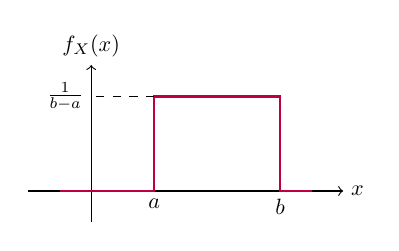
\begin{tikzpicture}[scale=0.8, transform shape]
            \draw[->] (-1,0) -- (4,0) node[right] {$x$};
            \draw[->] (0,-0.5) -- (0,2) node[above] {$f_X(x)$};
            \draw[thick, purple] (-0.5,0) -- (1,0) -- (1,1.5) -- (3,1.5) -- (3,0) -- (3.5,0);
            \draw[dashed] (1,1.5) -- (0,1.5) node[left] {$\frac{1}{b-a}$};
            \node[below] at (1,0) {$a$};
            \node[below] at (3,0) {$b$};
        \end{tikzpicture}
        \end{center}

        \begin{align*}
            \mu = \frac{a+b}{2} \qquad \qquad \sigma^2 = \frac{(b-a)^2}{12} \qquad \qquad \sigma = \frac{b-a}{\sqrt{12}}
        \end{align*}

    \subsubsection{Dreiecksverteilung}
        \textbf{Vorkommen:} Entsteht durch Faltung (Summe) von zwei unabhängigen Gleichverteilungen. (Zwei Würfel) 
        \begin{center}
        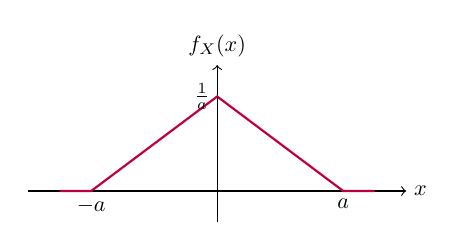
\begin{tikzpicture}[scale=0.8, transform shape]
            \draw[->] (-3,0) -- (3,0) node[right] {$x$};
            \draw[->] (0,-0.5) -- (0,2) node[above] {$f_X(x)$};
            \draw[thick, purple] (-2.5,0) -- (-2,0) -- (0,1.5) -- (2,0) -- (2.5,0);
            \draw[dashed] (0,1.5) -- (0,0);
            \node[left] at (0,1.5) {$\frac{1}{a}$};
            \node[below] at (-2,0) {$-a$};
            \node[below] at (2,0) {$a$};
        \end{tikzpicture}
        \end{center}

        \begin{align*}
            \mu = 0 \qquad \qquad \sigma^2 = \frac{a^2}{6}
        \end{align*}

    \subsubsection{Normalverteilung (Gauss-Verteilung)}
        \textbf{Entstehung \& Vorkommen:} Viele unabhängige Einzelfehler, die sich aufsummieren (Zentraler Grenzwertsatz).
        \begin{center}
        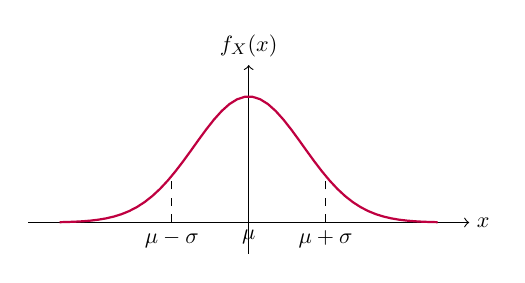
\begin{tikzpicture}[scale=0.8, transform shape]
            \draw[->] (-3.5,0) -- (3.5,0) node[right] {$x$};
            \draw[->] (0,-0.5) -- (0,2.5) node[above] {$f_X(x)$};
            % draw gaussian: e^(-x^2/1.5) * 2
            \draw[thick, purple, domain=-3:3, samples=50] plot (\x, {2*exp(-(\x*\x)/1.5)});
            % sigma approx at x=1.22
            \draw[dashed] (1.22,0) -- (1.22,{2*exp(-(1.22*1.22)/1.5)});
            \draw[dashed] (-1.22,0) -- (-1.22,{2*exp(-(1.22*1.22)/1.5)});
            \node[below] at (0,0) {$\mu$};
            \node[below] at (1.22,0) {$\mu+\sigma$};
            \node[below] at (-1.22,0) {$\mu-\sigma$};
        \end{tikzpicture}
        \end{center}

        \textbf{Vorgehen mit dem Taschenrechner (Fakultätsrechner, Menü 7):}
        \begin{itemize}
            \item \textbf{7.1 Normal-Dichte ($f(x)$):} Berechnet den y-Wert der Gaussglocke. (Wird für Wahrscheinlichkeiten \textbf{nicht} benutzt!)
            \item \textbf{7.2 Normal-Vert ($P(x_1 < X < x_2)$):} Berechnet die gesuchte Wahrscheinlichkeit (Fläche) für ein Intervall. 
            \begin{itemize}
                \item \textbf{Eingaben für 7.2:}
                \item \texttt{Lower}: Untere Grenze des gesuchten Intervalls
                \item \texttt{Upper}: Obere Grenze des gesuchten Intervalls
                \item \texttt{$\sigma$}: Standardabweichung
                \item \texttt{$\mu$}: Mittelwert
            \end{itemize}
            Geht ein Intervall bis unendlich, einfach einen sehr grossen Wert (z.B. $10^{99}$) bei Upper bzw. $-10^{99}$ bei Lower eingeben.
        \end{itemize}

\subsection{Rechnen mit Zufallsvariablen}
    \subsubsection{Kovarianz und Korrelation}
        Beschreibt die lineare Abhängigkeit zwischen zwei Messreihen $X$ und $Y$:
        \begin{align*}
            \text{Kovarianz: } \operatorname{Cov}(X,Y) &= E\{(X - \mu_X)(Y - \mu_Y)\} \\
            \text{Korrelationskoeffizient: } \rho(X,Y) &= \frac{\operatorname{Cov}(X,Y)}{\sigma_X \cdot \sigma_Y}
        \end{align*}
        \textit{Für unkorrelierte (unabhängige) Messungen gilt immer: $\operatorname{Cov}(X,Y) = 0$}

        \textbf{Wichtige Rechenregeln der Kovarianz:}
        \begin{itemize}
            \item \textbf{Gemeinsamer systematischer Fehler (Bias):} Besitzen zwei Messungen $X$ und $Y$ denselben zufälligen systematischen Fehler $B$ (mit Varianz $\sigma_B^2$) und ansonsten unabhängige Fehler $e_X, e_Y$ (also $X = \mu_X + B + e_X$ und $Y = \mu_Y + B + e_Y$), so ist die Kovarianz gleich der Varianz des Bias:
            \[ \operatorname{Cov}(X,Y) = \operatorname{Cov}(B,B) = \sigma_B^2 \]
            \item \textbf{Überlappende Messwerte (z.B. gleitender Mittelwert):} Bestehen zwei abgeleitete Größen aus linear kombinierten unabhängigen Messwerten, bei denen einige Werte in beiden vorkommen (z.B. $Y_1 = \frac{X_1 + X_2}{2}$ und $Y_2 = \frac{X_2 + X_3}{2}$), ergibt sich die Kovarianz nur aus den gemeinsamen Elementen:
            \[ \operatorname{Cov}(aX_1 + bX_2, cX_2 + dX_3) = b \cdot c \cdot \sigma_{X_2}^2 \]
            Für das Beispiel des gleitenden Mittelwerts: $\operatorname{Cov}(Y_1, Y_2) = \frac{1}{2} \cdot \frac{1}{2} \cdot \sigma_{X_2}^2 = \frac{1}{4}\sigma_{X_2}^2$
            \item \textbf{Allgemeine Rechenregeln:}
            \begin{align*}
                \operatorname{Cov}(X,X) &= \sigma_X^2\\
                \operatorname{Cov}(aX, bY) &= a \cdot b \cdot \operatorname{Cov}(X,Y) \\
                \operatorname{Cov}(X+Y, Z) &= \operatorname{Cov}(X,Z) + \operatorname{Cov}(Y,Z)
            \end{align*}
        \end{itemize}

    \subsubsection{Addition von korrelierten Messfehlern}
        Werden zwei Messungen $X$ und $Y$ gewichtet addiert ($Z = a \cdot X + b \cdot Y$):
        \begin{align*}
            \sigma_Z^2 &= a^2 \cdot \sigma_X^2 + 2 \cdot a \cdot b \cdot \operatorname{Cov}(X,Y) + b^2 \cdot \sigma_Y^2
        \end{align*}
        Spezialfälle für Korrelationskoeffizient $\rho$:
        \begin{itemize}
            \item \textbf{Vollständig korreliert} ($\rho=1$): $\operatorname{Cov}(X,Y) = \sigma_X \cdot \sigma_Y$
            \item \textbf{Unkorreliert} ($\rho=0$): $\operatorname{Cov}(X,Y) = 0$
            \item \textbf{Vollständig entgegengesetzt} \\
            ($\rho=-1$): $\operatorname{Cov}(X,Y) = -\sigma_X \cdot \sigma_Y$
        \end{itemize}

    \subsubsection{Addition von unabhängigen Messfehlern}
        Werden zwei unkorrelierte Messungen $X$ und $Y$ addiert ($Z = X + Y$):
        \begin{align*}
            \mu_Z &= \mu_X + \mu_Y \\
            \sigma_Z^2 &= \sigma_X^2 + \sigma_Y^2 \qquad \text{(Varianzen addieren sich!)} \\
            \sigma_Z &= \sqrt{\sigma_X^2 + \sigma_Y^2}
        \end{align*}

    \subsubsection{Multiplikation mit einer Konstanten}
        Multiplikation der Zufallsvariablen $X$ mit einer Konstanten ($Y = a \cdot X$).
        
        Mittelwert:
        \begin{align*}
            \mu_Y &= E\{Y\} = E\{a \cdot X\} = a \cdot E\{X\} = a \cdot \mu_X
        \end{align*}
        Varianz:
        \begin{align*}
            \sigma_Y^2 &= a^2 \cdot \sigma_X^2
        \end{align*}
        \begin{align*}
            \sigma_Y &= |a| \cdot \sigma_X
        \end{align*}

    \subsubsection{Fehlerfortpflanzung bei nichtlinearen Funktionen}
        Wird ein Messwert in eine nichtlineare Funktion $f$ eingesetzt, kann die Varianz mit Hilfe der ersten Ableitung (Linearisierung) an der Stelle des Mittelwerts genähert werden.
        \begin{itemize}
            \item \textbf{Eindimensional} ($Z = f(X)$):
            \begin{align*}
                \mu_Z &\approx f(\mu_X) \\
                \sigma_Z^2 &\approx \left(\frac{\partial f}{\partial x}\bigg|_{\mu_X}\right)^2 \cdot \sigma_X^2 \\
                \sigma_Z &\approx \left|\frac{\partial f}{\partial x}\bigg|_{\mu_X}\right| \cdot \sigma_X
            \end{align*}
            \item \textbf{Mehrdimensional} ($Z = f(X,Y)$ für unabhängige Variablen):
            \begin{align*}
                \mu_Z &\approx f(\mu_X, \mu_Y) \\
                \sigma_Z^2 &\approx \left(\frac{\partial f}{\partial x}\bigg|_{\mu_X, \mu_Y}\right)^2 \cdot \sigma_X^2 + \left(\frac{\partial f}{\partial y}\bigg|_{\mu_X, \mu_Y}\right)^2 \cdot \sigma_Y^2
            \end{align*}
        \end{itemize}

    \subsubsection{Mittelung von Messwerten}
        Werden $N$ unabhängige Messungen derselben Grösse gemittelt ($Z = \frac{1}{N}\sum_{i=1}^{N} X_i$):
        \begin{align*}
            \mu_Z &= \mu_X \\
            \sigma_Z^2 &= \frac{1}{N} \cdot \sigma_X^2 \qquad \text{(Die Varianz sinkt um den Faktor } N \text{)} \\
            \sigma_Z &= \frac{\sigma_X}{\sqrt{N}} \qquad \text{(Die Standardabweichung sinkt um } \sqrt{N} \text{)}
        \end{align*}

    \subsubsection{Schätzung von Mittelwert und Varianz aus einer Stichprobe}
        Liegt eine endliche Stichprobe mit $N$ Werten vor, können Mittelwert und Varianz geschätzt werden.
        \begin{itemize}
            \item \textbf{Schätzung des Mittelwerts:}
            \begin{align*}
                \hat{\mu}_X &= \frac{1}{N} \sum_{n=0}^{N-1} x_n \qquad \qquad \text{Standardabweichung des Mittelwerts: } \sigma_\mu = \frac{\sigma_X}{\sqrt{N}}
            \end{align*}
            \item \textbf{Schätzung der Varianz (wahrer Mittelwert $\mu_X$ bekannt):}
            \begin{align*}
                \hat{\sigma}_X^2 &= \frac{1}{N} \sum_{n=0}^{N-1} (x_n - \mu_X)^2
            \end{align*}
            \item \textbf{Schätzung der Varianz (Mittelwert $\hat{\mu}_X$ ebenfalls aus Stichprobe ermittelt):}
            \begin{align*}
                \hat{\sigma}_X^2 &= \frac{1}{N-1} \sum_{n=0}^{N-1} (x_n - \hat{\mu}_X)^2
            \end{align*}
        \end{itemize}

    \subsubsection{Zentraler Grenzwertsatz}
        Die Summe oder der Mittelwert einer großen Anzahl $N$ von unabhängigen Zufallsvariablen (mit Mittelwert $\mu$ und Varianz $\sigma^2$) nähert sich für große $N$ einer Normalverteilung an, \textbf{unabhängig davon, wie die einzelnen Variablen verteilt sind}.
        
        \begin{align*}
            \text{Summe } Z = \sum_{i=1}^{N} X_i \quad &\implies \quad Z \sim \mathcal{N}(N \cdot \mu, N \cdot \sigma^2) \\[1ex]
            \text{Mittelwert } \overline{X} = \frac{1}{N}\sum_{i=1}^{N} X_i \quad &\implies \quad \overline{X} \sim \mathcal{N}\left(\mu, \frac{\sigma^2}{N}\right)
        \end{align*}
        \textit{Dies ist der Grund, warum Messfehler, die aus vielen kleinen, unabhängigen Ursachen bestehen, in der Praxis meistens normalverteilt sind (Gauß-Verteilung).}

    \subsubsection{Sensorfusion / Optimale Gewichtung}
        Kombiniert man zwei unabhängige Sensormessungen linear ($Z = a \cdot X + b \cdot Y$), so gilt:
        \begin{align*}
            \mu_Z &= a \cdot \mu_X + b \cdot \mu_Y \\
            \sigma_Z^2 &= a^2 \cdot \sigma_X^2 + b^2 \cdot \sigma_Y^2
        \end{align*}
        Für eine echte gewichtete Mittelung gilt: $a+b = 1 \implies b = 1-a$. \\
        optimale Gewichtung: $\frac{\partial \sigma_Z^2}{\partial a} \stackrel{!}{=} 0$.     
        \begin{align*}
            \frac{\partial \sigma_Z^2}{\partial a} = 2a \cdot \sigma_X^2 - 2(1-a) \cdot \sigma_Y^2 \stackrel{!}{=} 0\\
            a = \frac{\sigma_Y^2}{\sigma_X^2 + \sigma_Y^2} \qquad \text{und} \qquad b = 1-a = \frac{\sigma_X^2}{\sigma_X^2 + \sigma_Y^2}
        \end{align*}
        \textbf{minimale Varianz}:
        \begin{align*}
            \sigma_{Z,opt}^2 = \frac{\sigma_X^2 \cdot \sigma_Y^2}{\sigma_X^2 + \sigma_Y^2} 
        \end{align*}

    \subsubsection{Auswirkung von digitalen Filtern auf Messrauschen}
        Wird ein verrauschtes Signal $x[n]$ mit unkorreliertem Rauschen (Varianz $\sigma_X^2$) durch ein digitales Filter mit der Impulsantwort $h[m]$ gefiltert, berechnet sich die Varianz des Ausgangsrauschens $\sigma_Y^2$ zu:
        \begin{align*}
            \sigma_Y^2 &= \sigma_X^2 \cdot \sum_{m=-\infty}^{\infty} (h[m])^2
        \end{align*}
